%
% Manchester Raspberry Jam Workshop Booklet
%
% This template is designed to try and aide consistency between each booklet.
% Insert files and settings only as instructed by comments.
%

% Is this document PRINT or WEB format?
% use \printtrue or \printfalse
\newif\ifprint
\printtrue

% Page Formatting
\ifprint
	\documentclass[a4paper, twocolumn, twoside, 11pt]{article}
	\usepackage[margin=2cm]{geometry}
	\setlength{\columnsep}{1.25cm}
	\setlength{\parskip}{6pt}
\else
	\documentclass[a4paper, onecolumn, oneside, 11pt]{article}
	\usepackage[margin=3cm]{geometry}
	\setlength{\parskip}{9pt}
\fi



% FONT and text format
\usepackage[utf8x]{inputenc}	
\usepackage[UKenglish]{babel}
\ifprint
	\usepackage[usenames, dvipsnames]{color}				%Font Colour
	\usepackage[colorlinks=false]{hyperref}	%URLs
\else
	\usepackage[T1]{fontenc}
	\usepackage[sfdefault]{roboto}
	\usepackage[T1]{fontenc}
	\usepackage[usenames, dvipsnames]{color}				%Font Colour
	\usepackage[colorlinks=true,linkcolor=black,urlcolor=WildStrawberry]{hyperref}
\fi



% Table of Contents Format
\usepackage{tocloft}
\addtocontents{toc}{\cftpagenumbersoff{subsection}}
\setcounter{tocdepth}{2}
\setcounter{secnumdepth}{2}



% Section spacing
\ifprint
	\usepackage[compact]{titlesec}
\fi



% Listings and Asides
\usepackage{McrRaspJam/common/listings}
\usepackage{McrRaspJam/common/asides}



%Clear page for web version
\newcommand{\webclearpage}{
	\ifprint
	\else
		\clearpage
	\fi
}

% misc.
\usepackage{enumitem}									%List spacing changes
\usepackage[toc,page]{appendix}							%Appendix package
\usepackage{graphicx}									% TOC?
\usepackage{etoolbox}									%Boolean used for print/web switching
\usepackage{fancyvrb}									%Centered verbatim

% Enter the document title here
\newcommand{\workshopTitle}{Workshop 16: Ciphers}

% Enter the author of this workshop
\newcommand{\workshopAuthor}{Written by Jack Kelly}


\begin{document}
	% Title Format
\ifprint
	\title{Manchester Raspberry Jam \\ \workshopTitle}
	\author{}
\else
	\title{
		\begin{center}
			
\includegraphics[width=30mm]{McrRaspJam/common/logo-512}
		\end{center}
		\vspace{12pt}
		\workshopTitle
	}
	\author{
		Written by \workshopAuthor
	}
\fi

\date{\vspace{-16pt}}
\maketitle


% Online download location
\ifprint
	\begin{mdframed}[rightline=false, leftline=false]
		\scriptsize
		This booklet is available online at \mbox{\href{https://drive.google.com/open?id=0B_1SFjX_5JrmfnhpX0pPRXl6bmJNal8zdUxMeWZOdjJyZVdzU3V6UnBGdlVIMENtbFFkbVk}{bit.ly/McrRaspJam}}
		\normalsize
	\end{mdframed}
\fi
	
	%Place a SINGLE paragraph summary here
	Learn how classical ciphers worked, and how to write Python programs to encode, decode and crack them!
	
	%Difficulty
	\textit{Difficulty: Introductory workshop.}
	
	\ifprint
		\renewcommand{\baselinestretch}{0.75}\normalsize
		\tableofcontents
		\renewcommand{\baselinestretch}{1.0}\normalsize
	\else
		\tableofcontents
	\fi
	
	%
	% Input the main CONTENT below, sans title page or contents.
	% Recommend inputting per section, and adding page breaks here.
	%
	% \webclearpage command is provided, will break page for web format only.
	%
	
	\setcounter{section}{-1}
\section{Introduction}

	Last month in \href{http://mcrraspjam.org.uk/workshop-15-gpio-zero/}{workshop 15}, we \textit{encoded} a message in Morse code, a method that makes it simpler to transmit written language through rudimentary means, such as a spotlight, or a pulse in an electrical wire.
	
	We also often use the word \textit{code} to refer to an encrypted \textbf{cipher}. A different type of encoding, when we encode a message in a cipher, we attempt to make the message difficult---or ideally impossible--- for an outsider to read.
	
	Today, we'll have a go at encoding, decoding and cracking some famous ciphers of the classical era using Python programs, as well as taking a look at more modern ciphers and some of the cryptography tools available to us as users of Linux on the Raspberry Pi.
	
	
	%Difficulty
	This is an introductory workshop, all of the Python concepts will be covered from scratch.
		
	\subsection*{How to use these booklets}

	The aim of these booklets is to help you attempt these workshops at home, and to explain concepts in more detail than at the workshop. You don't need to follow these booklets during the workshop, but you can if you'd like 0to.
	
	%Code Listings
		When you need to make changes to your code, they'll be presented in \textit{listings} like the example below. Some lines may be repeated across multiple listings, so check the line numbers to make sure you're not copying something twice.

	\lstinputlisting[style=Python, lastline=2]{McrRaspJam/015_GPIOZero/0_introduction/led.py}
	
	
	
	Occasionally, a concept will be explained in greater detail in \textit{asides}, like the one below. You can read these as you wish, but they're not required to complete the workshop.
	
\begin{aside}[Resistors]
	Resistors are most commonly used to limit the amount of current flowing through part of an electrical circuit.
	
	For example we use resistors in series with LEDs, as otherwise they could draw so much power that they destroy themselves.
	
	Buttons have almost no internal resistance, so we use high value ($\sim 10  k\Omega$) resistors to prevent current flowing straight from the power supply to ground; if we didn't, the entire CPU could be short circuited, and the Pi would lose power!
\end{aside}
	
	\ifprint\else
		\subsection*{What you'll need}
		All of the software you for this workshop is pre-installed on recent versions of Raspbian.
	\fi
		
	\subsection*{Everything else}
	
		% Aknowledgements
		These booklets were created using \textrm{\LaTeX}, an advanced typesetting system used for several sorts of books, academic reports and letters.
			
		\ifprint\else If you'd like to have a look at using LaTeX, We recommend looking at \TeX studio, which is available on most platforms, and also in the Raspbian repository. \fi
		
		% License spiel
		To allow modification and redistribution of these booklets, they are distributed under the \hbox{CC BY-SA 4.0} License.
		Latex source documents are available at \url{http://github.com/McrRaspJam/booklet-workshops}
		
		If you get stuck, find errors or have feedback about these booklets, please email me at:
		\href{mailto:jam@jackjkelly.com}{\texttt{jam@jackjkelly.com}}
	\clearpage
	
	\section{Python Basics}

	In order to write programs to perform cryptography, we will need to be able to manipulate words and sentences, which in programming we call \textit{strings}.
	
	We'll start with some basic Python programs, which will teach us everything we need in order to pull words and sentences apart.
	
	\begin{figure}[h]
		\centering
		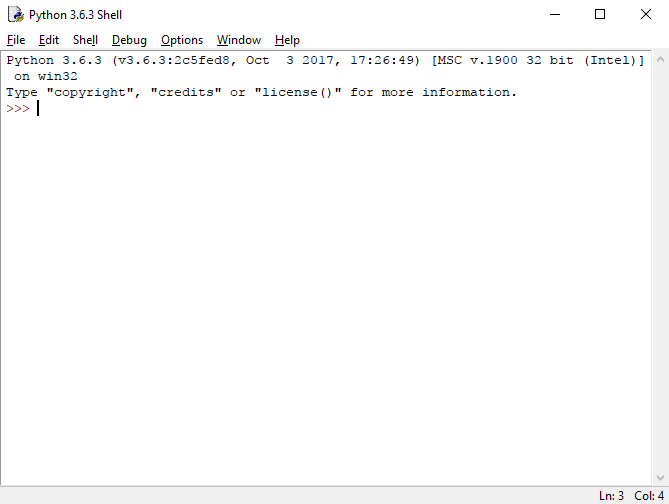
\includegraphics[width=0.8\linewidth]{McrRaspJam/016_Ciphers/1_python/idle}
		\caption{The IDLE \textit{shell} window}
		\label{fig:idle}
	\end{figure}
	
	Go to the main menu on your Raspberry Pi desktop and \textbf{open} the application titled \textit{Python 3 (IDLE)}.
	
	After a few seconds, IDLE will open to the \textit{Python Shell}. In this window, go to \textbf{File $\rightarrow$ New File}, which will open an empty window where we can write our programs.
	
	\subsection*{Hello, World!}
		
		In your empty window, \textbf{copy} the following program:
		
		\lstinputlisting[style=Python, title=helloworld.py]{McrRaspJam/016_Ciphers/1_python/helloworld.py}
		
		then, select \textbf{Run $\rightarrow$ Run Module} at the top of the window.
		
		After saving, your program will run and ``Hello, World!'' should appear in the shell window in blue.
		
	\subsection*{Inputting text}
	
		The next thing we'll need for our cipher programs is to enter text when our program runs. \textbf{Modify} your code to add the following command.
		
		\lstinputlisting[style=Python]{McrRaspJam/016_Ciphers/1_python/input.py}
		
		\textbf{Run} your program again. This time you will be asked to enter text into the shell window, and when you press enter it will be repeated back to you.
		
		\begin{aside}[Variables]
			When we store data (like text or numbers) in our programs, we store them as \textit{variables}.
			
			A variable has a \textit{label}---what the variable is called---and a \textit{value}---the data we wish to store in it.
			
			When we `set' a variable, we call this an \textit{assignment}, signified by the \texttt{=} sign.
		\end{aside}
	
	\subsection*{Lists}
	
		It is often useful to store several pieces of data in a single variable. A common way of doing this in Python is to use a list.
		
		\textbf{Open} a new file by selecting \textbf{File $\rightarrow$ New File}, then write the following program in the new window:
		
		\lstinputlisting[style=Python, title=list.py, breaklines=true]{McrRaspJam/016_Ciphers/1_python/list.py}
		
		Before you run your program, have a guess what will be printed out when you run the program. Run your program, then see whether what was printed matched what you thought it would be.
		
		\textit{extra challenge:} How can we fix the word spacing in the printed text?
		
		\begin{aside}[Lists]
			When we add \textit{elements} of data to a list, they are given the next available \textit{index} number.
			
			\vspace{4pt}
			\begin{tabular}{c|c}
				0 & Vanilla \\ 
				1 & Strawberry \\ 
				2 & Chocolate \\ 
				3 & Raspberry Ripple
			\end{tabular} 
			\vspace{4pt}
						
			To access a single element from a list, we use square brackets, as we have done in our program above.
		\end{aside}
	
	\subsection*{Strings are Lists}
	
		When we write our cipher programs, we'll need to look at single letters from the sentences we input. In python, a text \texttt{string} is actually a list of single \texttt{characters}.
		
		This means that we can access a string just like a list. Return to your hello world program, and \textbf{modify} the print statement as follows.
	
		\textbf{\lstinputlisting[style=Python, title=helloworld.py]{McrRaspJam/016_Ciphers/1_python/inputlist.py}}
		
		Now, when you run your program, only the first letter of whatever you typed in will be printed out.
		
		Next, we'll try printing out each letter one-by-one, which we can do using a \textit{loop}.
		
		\textbf{\lstinputlisting[style=Python, title=helloworld.py]{McrRaspJam/016_Ciphers/1_python/inputlist2.py}}
		
		The \texttt{for} loop we used repeats once for each element in the list that we provide it, in this case each letter in our string.
		
		\textbf{Run} your program, and this time your text should be printed one character at a time, each on its own line.
		
	\webclearpage
	
	\section{Substitution Ciphers}

	\ifprint\else	
		Ciphers have existed in some form since the classical era. One of the earliest examples of ciphers being used to keep information are clay tablets from Mesopotamia---dating back to 1500 BCE---which were used to keep trade secrets like the recipe for pottery glaze.
	
		\begin{aside}[Origins of Ciphers]
			From \href{http://en.wikipedia.org/wiki/History_of_cryptography}{Wikipedia}:
			
			\textit{``The earliest known use of cryptography is found in non-standard hieroglyphs carved into the wall of a tomb from the Old Kingdom of Egypt circa 1900 BCE.}
				
			\textit{``These are not thought to be serious attempts at secret communications, however, but rather to have been attempts at mystery, intrigue, or even amusement for literate onlookers.''}
		\end{aside}
	\fi
	
\subsection{Atbash}

	Atbash was a simple substitution cipher that emerged around 500 BCE, and was originally used to encode the Hebrew alphabet.
	\ifprint\else (the name is a shortening of the letters Aleph-Tav-Beth-Shin) \fi
	
	In a substitution cipher, the characters of the plain-text are \textit{substituted} with another set of characters---usually the same alphabet in a different order. For Atbash, this is very simple, the alphabet is reversed.
	
	\begin{figure*}
		\begin{tabular}{r|cccccccccccccccccccccccccc}
			\textbf{plaintext} & a & b & c & d & e & f & g & h & i & j & k & l & m & n & o & p & q & r & s & t & u & v & w & x & y & z \\ 
			\hline
			\textbf{ciphertext} & z & y & x & w & v & u & t & s & r & q & p & o & n & m & l & k & j & i & h & g & f & e & d & c & b & a \\ 
		\end{tabular} 
		\caption{Atbash substitution for the Latin alphabet}
		\label{fig:atbash}
	\end{figure*}

	\subsubsection*{An Example}
	
		The tradition when practising cryptography is to use faux military commands, so we'll start with the plaintext ``\textbf{Attack at dawn}''.
		
		using the table in \autoref{fig:atbash}, we find each letter in the first row, and replace it with the letter in the following row.
		
		\begin{tabular}{ccc}
			A & $\rightarrow$ & Z \\ 
			t & $\rightarrow$ & g \\ 
			t & $\rightarrow$ & g \\ 
			a & $\rightarrow$ & z \\ 
			c & $\rightarrow$ & x \\ 
			k & $\rightarrow$ & p \\ 
		\end{tabular} 
	
		Our ciphertext for this phrase would be ``\textbf{Zggzxp zg wzdm}''.
	
		Now, using a pen and paper and \autoref{fig:atbash}, have a go at encoding the following plaintext using Atbash.
		
		``\textbf{We are discovered, flee at once}''
	
	\subsubsection*{Atbash in Python}
	
		Now we know how Atbash works, we can try writing a Python program that encodes it.
		
		When run in a terminal, the program should look like the following:
		
		\begin{lstlisting}[style=Terminal, numbers=none]
$ python3 atbash.py
Enter plaintext: attackatdawn
zggzxpzgwzdm
		\end{lstlisting}
		
		\textbf{Open} a new script file in IDLE by going to \texttt{File $\rightarrow$ New File}.
		
		The first thing our program needs to do when run is get the plaintext. We'll use an \texttt{input()} function, just like we did in \autoref{python}.
		
		\lstinputlisting[style=Python, lastline=1, title=atbash.py]{McrRaspJam/016_Ciphers/2_ciphers1/atbash1.py}
		
		We'll also set an empty \texttt{string} variable, where we'll add our ciphertext.
		
		\lstinputlisting[style=Python, firstline=2, firstnumber=2]{McrRaspJam/016_Ciphers/2_ciphers1/atbash1.py}
	
		The other thing we need is a copy of the table in \autoref*{fig:atbash}, which we'll place in lists.
		
		We could do this by manually defining the list:
		
		\lstinputlisting[style=Python, numbers=none, breaklines=true, lastline=1]{McrRaspJam/016_Ciphers/2_ciphers1/alphabetlist.py}
		
		but let's save some time and take advantage of one of Python's libraries to automate the generation of this list:
		
		\lstinputlisting[style=Python, lastline=6]{McrRaspJam/016_Ciphers/2_ciphers1/atbash2.py}
		
		Then we'll create the substitute alphabet by copying the list in reverse:
		
		\lstinputlisting[style=Python, firstline=7, firstnumber=7, lastline=7]{McrRaspJam/016_Ciphers/2_ciphers1/atbash2.py}
		
		\ifprint\else You can check these lists are correct by running the program, then typing \texttt{alphabet} and \texttt{subalphabet} into the shell window prompt, which will print their contents. \fi
	
		We have everything we need, we can now perform the encryption. Just like on pen and paper, we convert each letter one-by-one, so we'll use the loop we learned in \autoref{python}.
	
		\lstinputlisting[style=Python, firstline=8, firstnumber=8, lastline=9]{McrRaspJam/016_Ciphers/2_ciphers1/atbash2.py}
		
		\pagebreak[3] %pagebreak hint
		
		%\textbf{Look away} from your program for the moment.
		
		At this point we have one more problem to consider. To pull a letter from the alphabet list, we need to access it using an index number. (In \texttt{alphabet} 0=a, 1=b, 2=c, etc.)
		
		We need a way to number letters based on their position in the alphabet. Fortunately, the ASCII encoding scheme already assigns a number to each letter, and because it is widely used it is very easy to get the  code for a letter in Python.
		
		\pagebreak[2] %pagebreak hint
		
		\begin{aside}[ASCII]
			ASCII (\textit{American Standard Code for Information Interchange}) was invented as a way to standardise how letters were stored on different file formats and computer systems, starting in the early 1960's.
			
			ASCII encodes a small number of characters, mostly, alphanumeric characters, punctuation and control characters (things like `new line', `end of file' or `backspace'.)
			
			These days, most text is actually encoded in the much larger \href{https://unicode.org/}{Unicode} standard.
		\end{aside}
		
		To get a number for each letter in our loop:
		
		\begin{lstlisting}[style=Python, firstnumber=9]
for letter in plaintext:
    charnumber = ord(letter)
		\end{lstlisting}
		
		However, the ASCII number for ``a'' is `97', ``b'' is `98' etc. so we'll need to subtract 97 to match the 0--25 range of our alphabet list 
		
		\lstinputlisting[style=Python, firstline=10, firstnumber=10, lastline=10]{McrRaspJam/016_Ciphers/2_ciphers1/atbash2.py}
		
		Now, we can simply take the character number, and access the substitute alphabet list using the same index.
		
		\begin{lstlisting}[style=Python, firstnumber=11]
    subalphabet[charnumber]
		\end{lstlisting}
		
		Remember that we're in a loop, so we just need to add the current cipher letter to the ciphertext.
		
		\lstinputlisting[style=Python, firstline=11, firstnumber=11, lastline=11]{McrRaspJam/016_Ciphers/2_ciphers1/atbash2.py}
		
		Once the loop has completed, our ciphertext should be complete! We simply need to add a print statement outside of the loop.
		
		\lstinputlisting[style=Python, firstline=11, firstnumber=11]{McrRaspJam/016_Ciphers/2_ciphers1/atbash2.py}
		
		Try testing the program using the two plaintexts from the pen and paper exercise and see if the output from your program matches.
		
		Bear in mind your program currently has some limitations:
		\begin{itemize}[nosep]
			\item Capital letters won't work, as they have different ASCII codes to lowercase letters.
			\item We haven't told the program what to do with spaces, so we can't use them either.
		\end{itemize}
	
		If you wanted to extend your program, fixing these would be a good place to start. You should also have a think about the following:
		
		\begin{itemize}[nosep]
			\item Our program currently \textit{encodes} Atbash ciphers. What would we have to do to write a program that \textit{decodes} the cipher?
			\item How secure do you think Atbash is?
		\end{itemize}	
	\subsection{Caesar Cipher}
	
	The Caesar cipher is another substitution cipher named after the Julius Caesar, who used it to encrypt messages of military significance.
	
	This cipher is similar to Atbash, but instead of reversing the alphabet, the substitute alphabet is created by shifting letters.
	
	\begin{figure}[h]
		\centering
		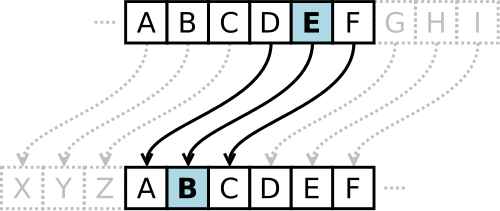
\includegraphics[width=0.5\linewidth]{McrRaspJam/016_Ciphers/2_caesar/caesarshift}
		\caption{Shifting letters to create the substitute alphabet}
		\label{fig:caesardiagram}
	\end{figure}
	
	\subsubsection{An Example}
	
		If we wish to encrypt the plaintext ``\textbf{The enemy surrounds us}'' with a rightward shift of \textbf{1} place, we can use the table in \autoref{fig:caeser} as follows:
		
		\begin{tabular}{ccccccc}
			T & $\rightarrow$ & u && e & $\rightarrow$ & f \\ 
			h & $\rightarrow$ & i && n & $\rightarrow$ & o \\ 
			e & $\rightarrow$ & f && e & $\rightarrow$ & f\\ 
			 & & && m & $\rightarrow$ & n\\ 
			 & & && y & $\rightarrow$ & z\\
		\end{tabular}
	
		Our full ciphertext for this phrase would be ``\mbox{\textbf{Uif fofnz tvsspvoet vt}}''.
		
		Returning to your pen and paper, have a go at encoding the following phrase.
		
		``\textbf{Attack from the west}'', right shift of \textbf{3}.
		
		Then try the following. You will need to construct your own substitute alphabet for this:
		
		``\textbf{The city has fallen}'', \textit{left} shift of \textbf{2}.
		
		\begin{figure*}
			\begin{tabular}{r|cccccccccccccccccccccccccc}
				\textbf{plaintext} & a & b & c & d & e & f & g & h & i & j & k & l & m & n & o & p & q & r & s & t & u & v & w & x & y & z \\ 
				\hline
				\textbf{Right 1} & b & c & d & e & f & g & h & i & j & k & l & m & n & o & p & q & r & s & t & u & v & w & x & y & z & a\\
				\textbf{Right 2} & c & d & e & f & g & h & i & j & k & l & m & n & o & p & q & r & s & t & u & v & w & x & y & z & a & b\\
				\textbf{Right 3} & d & e & f & g & h & i & j & k & l & m & n & o & p & q & r & s & t & u & v & w & x & y & z & a & b & c\\
			\end{tabular} 
			\caption{Caesar shift substitutions for the first three values of right shift}
			\label{fig:caeser}
		\end{figure*}

	\subsubsection*{Caesar Cipher in Python}
	
		Because the Caesar cipher is so similar to Atbash, we can reuse most of the code from that program.
		
		\textbf{Copy} the Atbash program---either through the file manager, or by \texttt{File $\rightarrow$ Save As...}---and rename, then open the new file.
		
		The first addition we will add to our program will be to allow the user to determine the shift for the cipher. We can do this with another \texttt{input()} function.
		
		\lstinputlisting[style=Python, title=caesar.py, firstline=3, firstnumber=3, lastline=6, breaklines=true]{McrRaspJam/016_Ciphers/2_caesar/caesar.py}
		
		Then, we need to create the substitute alphabet based on the shift number. This is more complex than Atbash, so we'll start with an empty list, and fill it using a loop.
		
		\lstinputlisting[style=Python, firstline=7, firstnumber=7, lastline=9]{McrRaspJam/016_Ciphers/2_caesar/caesar.py}
		
		To shift the letters, we'll first get the ASCII code for the letter and subtract 97, just like we did last time:
		
		\lstinputlisting[style=Python, firstline=10, firstnumber=10, lastline=13]{McrRaspJam/016_Ciphers/2_caesar/caesar.py}
		
		then we'll add the shift number. To wrap from one end of the alphabet to the other, we'll use a \textit{modulus} operator.
		
		\lstinputlisting[style=Python, firstline=14, firstnumber=14, lastline=14]{McrRaspJam/016_Ciphers/2_caesar/caesar.py}

		\ifprint\else
			\begin{aside}[Modulus Operation]
				The modulus operation (signified by \texttt{\%}) finds the remainder of a division.
				
				For the letter `x' (23)
				
				\begin{align*}
					23 \div 26 &= 0 \text{ remainder } \textbf{23}
				\end{align*}
				
				When shifted by 5, it `wraps around' to the start of the alphabet :
				
				\begin{align*}
					28 \div 26 &= 1 \text{ remainder } \textbf{2}
				\end{align*}
				
			\end{aside}
		\fi
		
		Finally, we grab the letter at this place in the alphabet, and add that to our substitute alphabet
		
		\lstinputlisting[style=Python, firstline=15, firstnumber=15, lastline=15, breaklines=true]{McrRaspJam/016_Ciphers/2_caesar/caesar.py}
		
		Your program should now be complete. Try encoding the phrases from the pen and paper examples, and see if they match.
		
		Have a think about the same questions we asked after we finished the Atbash program.
		
		\ifprint\else
			\begin{itemize}[nosep]
				\item Our program currently \textit{encodes} Caesar ciphers. What would we have to do to write a decoding program?
				\item What makes the Caesar cipher more secure than Atbash?
			\end{itemize}
		\fi

	\subsubsection*{Cryptographic Key}
	
		When we introduce a variable into an encryption method, we call this a cryptographic \textbf{key}. (sometimes called a \textit{cryptovariable})
		
		In Atbash, there is only one way that the alphabet is arranged, so there is no key. In the Caesar cipher, the cipher can be varied each time the cipher is used, so the shift number is the key for this cipher.
		
		\ifprint\else By introducing a key, an encrypted message can stay secure even if an intercepting party knows what cipher was used. However, the key \textit{must} be kept secret to maintain the security of the ciphertext. \fi

\subsection{Cracking the Caesar Cipher}

		If we don't hold the key to a ciphertext, we'll need to crack the code to access the plaintext.
		
		Because of the amazing computing speed of our Raspberry Pi, the easiest way to do this is to try every possible key in turn until we find the plaintext.
		
		\textbf{Open} the file \texttt{crackcaesar.py}, which contains a modified version of the program you just wrote.
		
		The program has been modified to use functions---which we will use shortly---and variable names have been switched to show that the program now goes from ciphertext to plaintext.
		
		The first modification we need is to make the decryption repeat to try each possible key. We'll place all of our previous code in a loop. (except for the input ciphertext)
		
		\lstinputlisting[style=Python, firstline=9, firstnumber=9, lastline=13, breaklines=true, title=crackcaesar.py]{McrRaspJam/016_Ciphers/2_caesar/crackcaesarb.py}
		
		We also need a way to tell when the solution has been found. To do this, we will check for the following suspect keywords: ``\textit{Attack}'', ``\textit{enemy}'', ``\textit{ally}'' and ``\textit{retreat}''.
		
		After generating each possible plaintext, we'll call the \texttt{check()} function. \textbf{Change} the following line:
	
		\begin{lstlisting}[style=Python, firstnumber=25]
print(plaintext)
		\end{lstlisting}
		
		to:
	
		\begin{lstlisting}[style=Python, firstnumber=25]
if check() == True:
	print(plaintext)
	break
		\end{lstlisting}
		
		The \texttt{check()} function will be very simple. It simply returns \texttt{True} if one of the words is found.
		
		\lstinputlisting[style=Python, firstline=28, firstnumber=28, lastline=30]{McrRaspJam/016_Ciphers/2_caesar/crackcaesara.py}
		
		Currently, the function always returns true, meaning the program always thinks it's found the solution on the first attempt.
		
		The following code returns true if the word ``attack'' is found in the possible plaintext. \textbf{Extend} the function to find the other 3 words.
		
		\begin{lstlisting}[style=Python, firstnumber=35]
def check():
	global plaintext
	found = False

	if "attack" in plaintext:
		found = True
		
	return found
		\end{lstlisting}
		
		Your program should now be complete. Try decoding the following ciphertexts:
		
		\begin{tabular}{c}
			``\textbf{jwljwslslgfuw}'' \\ 
			``\textbf{exxegoirvsyxi}''\\ 
			``\textbf{nbyyhygsulyxyzyunyx}''\\ 
			``\textbf{wjnsktwhjfqqdytxtzym}''\\
		\end{tabular} 
		
	\webclearpage

	\section{Transposition Ciphers}

	We've taken a look at substitution ciphers, when letters are replaced by other letters. Another common type of cipher is a \textit{transposition} cipher, where the letters stay the same, but are reordered in the ciphertext.

\subsection{Scytale}

	\begin{figure}[h]
		\centering
		
\includegraphics[width=0.7\linewidth]{McrRaspJam/016_Ciphers/3_transposition/Scytale}
		\caption{A scytale device}
		\label{fig:scytale}
	\end{figure}
	
	The scytale dates back to Ancient Greece and Sparta, and is a very simple to use device for encrypting methods.
	
	A person wishing to encrypt a message would simply wrap a long strip of parchment around the cylinder of the scytale and write their message across in rows. When unwrapped, the message would appear to be nonsense.
	
	\begin{itemize}[nosep]
		\item The scytale has a cryptographic key, what is it?
	\end{itemize}
	
	\begin{figure}[h]
		\centering
		
		\begin{tabular}{c|c|c|c|c}
			w & e & a & r & e \\ 
			\hline 
			d & i & s & c & o \\ 
			\hline 
			v & e & r & e & d \\ 
			\hline 
			h & e & l & p &  \\
		\end{tabular}
	
		\vspace{4pt}
		
		\begin{tabular}{ccccccccccccccccccc}
			w & d & v & h & e & i & e & e & a & s & r & l & r & c & e & p & e & o & d \\ 
		\end{tabular} 
	
		\caption{A scytale plaintext, and its unwrapped ciphertext}
		\label{fig:scytaletable}
	\end{figure}	
	
%	\begin{appendices}
%	\end{appendices}

\end{document}